% 這是我們研究室撰寫論文初稿的模板，已經整合了多個常用的 LaTeX 套件，並且提供了示例代碼，幫助學生快速上手。請根據需要修改和擴展這個模板，以適應不同的研究主題和投稿要求。
% 注意，請嚴格按照裡面指示撰寫你的論文，即便你已經使用出版社的 LaTeX 模板，也要確保裡面老師規定的要求都被滿足了，這樣才會節省我們雙方的時間，讓我們能夠專注在論文內容的改進上，而不是格式和基本要求上的問題。
\documentclass[11pt, a4paper]{article}

% ====== Preamble ======
% 引入自定義樣式檔
\usepackage{wmt-template}

% 引入可選套件
% microtype 提供了字距和行距的微調功能，可以提升整體的排版品質，當你的論文看起來長段落的文字過於擁擠或者行距不均勻時，microtype 可以幫助你自動調整字距和行距，使得整體的閱讀體驗更加舒適和專業。
% \usepackage{microtype}
% subcaption 提供了子圖和子表格的支持，讓我們能夠在同一個圖表環境中展示多個相關的圖像或表格，並且可以為每個子圖或子表格添加獨立的標題和說明。不過通常組圖我們會直接使用 script 畫圖來完成。
% \subsection{subcaption}

% 指定文獻資料庫路徑 (必須放在 Preamble 區塊)
\addbibresource{references.bib}

% 撰寫論文時將圖檔放在figures資料夾中，但是因為某些出版社的投稿系統需要平鋪圖檔在同一層級，所以我們在這裡設定優先搜索當前目錄，然後再搜索 figures 資料夾，這樣就能兼容不同的投稿要求。
\graphicspath{{./}{./figures/}} % 優先搜索當前目錄，再搜索 figures

% 自定義演算法關鍵字 (Optional)
% 詳請請見下面演算法範例中的使用說明，這些自定義的關鍵字可以幫助我們更清晰地表達演算法的流程和邏輯，提升演算法的可讀性和專業性。
\algnewcommand{\To}{\textbf{to }}
\algnewcommand{\Step}{\textbf{step }}

% 指定你的姓名，讓老師能知道是誰撰寫的論文，請直接寫英文名字，這個模板不支持中文。
\studentname{Student Name}

% 定義論文標題
\title{High-Performance Data Mining Framework for Large-Scale Systems}
\date{}

% ====== Main Content ======
% Abstract (摘要)
% 摘要是整篇論文的「電梯簡報」。審稿人與讀者通常只花 30 秒決定是否繼續閱讀。此處不應包含任何引用文獻或過於冷僻的縮寫。核心目標：用 200~250 字，清楚回答四個問題：Why (背景與問題), What (你的方法), How (技術核心), So What (結果與貢獻)。
% 內容檢核點：
% 第一句 (Context)：一句話點出領域現況與痛點（例如：隨著數據量指數級增長，傳統算法面臨記憶體瓶頸）。
% 第二句 (Problem)：明確指出目前 SOTA (State-of-the-Art) 方法的致命缺陷（例如：精確度不足、執行時間過長）。
% 第三句 (Proposed Method)：帶出我們提出的演算法名稱及其核心機制（例如：提出了 WMT-Miner，採用剪枝策略與並行架構）。
% 第四句 (Results)：提供具體的實驗數據證明（例如：實驗顯示，本方法在處理百萬級數據時，比 Baseline 快了 45%）。
% 寫作禁忌：
% 禁止使用模糊字眼（如 "very good", "much faster"），必須要有數字或具體形容詞。
% 禁止出現參考文獻編號（如 [1]）。

% Introduction (簡介)
% Introduction 採用「漏斗式」結構，由廣入深，最後收斂至本文貢獻。這是說服審稿人「這篇論文值得被接受」的關鍵戰場。
% 核心目標：建立研究的正當性 (Justification)，並明確條列出貢獻 (Contributions)。
% 內容檢核點：
% Background：簡述該研究議題在現代系統中的重要性。
% Research Gap (關鍵)：具體批判現有研究的不足。不要只說別人不好，要說「為什麼」不好（例如：無法擴展、忽略了某些邊界條件）。這能凸顯我們研究的必要性。
% Proposed Approach：高層次 (High-level) 地描述我們的解決方案。不用涉及數學細節，重點在於「設計哲學」（例如：我們採用了位元運算來優化空間）。
% Contributions (條列式，最少三點)：
% 第一點：提出了什麼新的架構或演算法。
% 第二點：解決了什麼具體技術難題（如：降低了時間複雜度從 O(n^2) 到 O(n log n)）。
% 第三點：進行了廣泛的實驗（包含真實數據與合成數據），證明了方法的強健性。
% 寫作禁忌：
% 禁止與 Abstract 內容完全複製貼上。
% 避免在 Contribution 中列出瑣碎的事項（如「我們寫了 Python code」不是貢獻，「開源了程式碼」才是）。
% 其他事項：
% 如果cite的文章的作者不只一位，請使用 et al.，但是 LaTex 的引擎會把逗點當作句子的結尾，所以一般我們會在et al.後面加上波浪符號（~）來避免這個問題，它會空出來的空格屬於句中空格的大小。
% 有時候老師會需要你在 Introduciton 中引用一些論文，請依照相關性放入「漏斗式」的結構中，從最廣泛的相關研究開始，逐漸聚焦到與我們研究最相關的文獻，最後引出我們的研究貢獻。
% 務必將我們的相關研究放入 Introduction 中，這樣才能讓審稿人清楚地看到我們的研究是建立在現有工作的基礎上，並且能夠明確地看到我們的貢獻和創新之處。

% Background (背景與相關研究)
% 此章節分為兩個子段落，功能截然不同。
% Related Work (相關研究)
% 核心目標：展現對領域的掌握度，並進行「分類批判」。寫作策略：
% 不要寫成流水帳（A 做了這，B 做了那）。
% 要進行分類：例如「基於樹結構的方法」有哪些，「基於矩陣的方法」有哪些。
% 總結缺點：每一類介紹完後，必須有一句總結，說明這類方法為何不能解決我們現在面對的問題（這就是我們存在的意義）。
% Preliminaries (預備知識與問題定義)
% 核心目標：定義戰場規則。所有後續用到的數學符號、資料結構定義，都必須在此處完成。內容檢核點：
% 基本定義 (Definitions)：定義什麼是資料庫 D、項目 I、閾值 delta。使用 LaTeX 的 definition 環境。
% 問題陳述 (Problem Statement)：用正式的數學語言描述輸入 (Input) 與輸出 (Output)。 Given... Find... Such that...
% 符號表 (Notations)：若符號較多，建議整理一個 Table 說明每個符號代表的意義。

% Proposed Algorithm (提出的演算法)
% 這是論文的技術核心（Heart of the paper）。
% 核心目標：清晰、無歧義地解釋你的演算法是如何運作的。
% 內容檢核點：
% 總體架構 (System Overview)：先給一張架構圖 (Architecture Diagram)，解釋數據流 (Data Flow) 是如何從輸入轉變為輸出。
% 核心策略 (Core Strategy)：詳細解釋演算法中的關鍵步驟（如：剪枝策略、候選生成、並行調度）。這部分需要配合數學公式證明其正確性。
% 虛擬碼 (Pseudocode)：使用 algorithm 與 algpseudocode 套件。
% 變數名稱必須與之前定義的一致。
% 每一行關鍵邏輯都要加上註解 (Comment)。
% 複雜度分析 (Complexity Analysis)：必須提供時間複雜度與空間複雜度的推導（最好有 Big-O notation）。這是系統類論文必備的防禦性論述。

% An Illustrated Example (圖解範例)
% 核心目標：降低閱讀門檻，證明演算法的可執行性。
% 寫作策略：
% 設計一個極簡的 Toy Dataset（例如只有 5 筆交易，4 個項目）。
% Step-by-Step：像是在白板上教學一樣，展示演算法在每一輪迭代後，資料結構（Table, Tree, Matrix）是如何變化的。
% 視覺化：每一各步驟最好配合圖表（Figure）或表格狀態（Sub-tables），讓審稿人不用看 Code 就能懂邏輯。

% Experimental Results (實驗結果)
% 核心目標：透過客觀數據證偽競爭對手，證明我方優勢。
% 內容檢核點：
% 實驗環境 (Setup)：清楚列出 CPU、RAM、作業系統、程式語言。
% 資料集 (Datasets)：列出使用的真實資料集與合成資料集，並提供其統計特徵（大小、維度、稀疏度）。
% 評估指標 (Metrics)：定義什麼是「好」？（執行時間、記憶體消耗、擴展性 Scalability）。
% 比較對象 (Baselines)：必須包含目前該領域公認的 SOTA 演算法。
% 圖表分析 (Analysis)：
% 不要只描述現象（如「A 比 B 高」）。
% 要解釋原因（如「A 比 B 高是因為 A 採用了索引機制，減少了 I/O」）。
% 必須包含：執行效率比較、記憶體使用量比較、可擴展性測試（Scalability test）。

% Conclusion and Future Works (結論與未來展望)
% 核心目標：總結價值，並展現學術誠實與前瞻性。
% 內容檢核點：
% 總結：用更宏觀的角度重述本文解決的問題與貢獻（不要跟 Abstract 字對字重複）。
% 管理意涵 (Managerial Implications)：(針對資管領域) 說明此技術對企業或系統管理的實際價值。
% 限制與未來 (Limitations & Future Works)：
% 誠實列出目前算法的限制（例如：不適用於串流數據）。
% 提出未來的改進方向（例如：引入 GPU 加速、結合聯邦學習等）。

% 其他需要注意的事項：
% 1. 現在論文撰寫的工具很多，所以不能接受有文法和拼字錯誤的論文，請務必使用 Grammarly 或是其他類似的工具來檢查你的論文，確保沒有明顯的語法錯誤和拼字錯誤，這樣才能提升論文的專業性和可讀性。
% 2. 雖然我不在意學生使用 AI 工具來協助撰寫論文，但是請務必確保論文的內容是你自己理解並且能夠解釋的，這樣才能在審稿過程中自信地回答審稿人的問題，並且在口頭報告中清晰地表達你的研究貢獻。不能無中生有，也不能抄襲他人的內容，這樣不僅會損害你的學術誠信，還可能導致論文被拒絕或者撤回。
% 3. 論文的結構和內容應該清晰且有邏輯性，避免出現重複的內容或者不相關的段落，這樣才能讓審稿人和讀者更容易理解你的研究工作，並且對你的貢獻有一個清晰的認識。
% 4. 在撰寫論文時，請務必遵守學術倫理和出版規範，確保所有引用的文獻都被正確地引用和列出，並且不要在論文中包含任何未經授權的內容或者侵犯他人版權的材料，這樣才能確保你的論文符合學術界的標準，並且能夠順利通過審稿過程。
% 5. 避免大章節 title 和小章節 title 之間完全沒有內容的情況，這樣會讓審稿人覺得你的論文結構不完整或者內容不充實，建議在每個章節之間至少有一段簡短的介紹或者過渡段落，這樣可以提升論文的流暢性和可讀性。
% 6. 避免出現主觀性詞語或者過於絕對的表達方式，例如 "we", "the best", "the most efficient", "always", "never" 等，這樣的表達可能會讓審稿人覺得你的論文缺乏客觀性和嚴謹性，建議使用更為謹慎和客觀的語言來描述你的研究成果。

\begin{document}

\maketitle
\thispagestyle{fancy}

\begin{abstract}
	In this paper, we present a high-performance data mining framework designed for large-scale systems. Our approach integrates advanced algorithms with optimized data structures to achieve superior performance. We demonstrate the effectiveness of our framework through extensive experiments on real-world datasets, showing significant improvements in both accuracy and efficiency compared to existing methods.
\end{abstract}

\section{Introduction}
This document demonstrates a modern LaTeX workflow optimized for academic research. By leveraging the \texttt{siunitx} package, we can ensure consistent formatting for numerical values and scientific units, such as \qty{180}{\celsius} or \unit{12}{ms}.

% cite指令如果要引用多篇文獻，可以使用逗號分隔，例如 \cite{Wu2024Systems,Wu2025ICDM}，這樣就能同時引用兩篇文獻，並且在參考文獻列表中顯示完整的引用信息。
% 注意，這個 sty 檔已經設定了 ref 數字會由小到大排序，並依照出現順序排列，不過出版社的模板可能會有不同的排序規則，而且可能不會自動排序，但是我們撰寫論文的時候還是要確定引用的數字是有經過排序的。
Citation example: According to \cite{Wu2024Systems,Wu2025ICDM}, the proposed method outperforms traditional approaches in terms of accuracy and computational efficiency.

% 以下為各個套件的使用範例，展示了它們在不同情境下的應用：
% 各套件已經被整合到 wmt-template.sty 中，學生在撰寫論文時可以直接使用這些功能，而不需要額外引入套件。
% 如果套用到出版社的 LaTeX 模板中，請確保不會與原有套件衝突，並且遵循出版社的格式要求。
% 出版社的模板若沒有包含這些套件，請自行添加到 preamble 區塊中。

% usepackage[dvipsnames]{xcolor} 範例，上色用，一般我們投稿以灰階為主，但是在撰寫、老師審閱階段和 revision 階段，使用顏色可以幫助我們更清晰地標註需要修改的部分或者強調重要的內容。
The \texttt{xcolor} package allows us to enhance the visual appeal of our documents by incorporating colors. For instance, we can highlight important results in tables or figures using predefined color names like \textcolor{red}{red} or \textcolor{blue}{blue}.
Ohter example, {\color{red} This part needs revision.} \colorbox{yellow}{Important note!} \fcolorbox{black}{azure9}{Target data} {\color{blue!60!white} Lighter blue}

% usepackage{enumitem} 範例
% 拿來羅列論文的貢獻，至少三點，並且每一點都要有詳細的說明，讓讀者能夠清楚地了解我們的研究貢獻。
The \texttt{enumitem} package provides extensive customization options for list environments. We can create nested lists with different styles, such as:
\begin{itemize}[label=\textbullet, leftmargin=2em]
	\item First level item
	      \begin{itemize}[label=\textendash, leftmargin=1.5em]
		      \item Second level item
		      \item Another second level item
	      \end{itemize}
	\item Another first level item
\end{itemize}

% usepackage{amsmath, amssymb, mathtools} 範例, amsmath 提供 LaTeX 最強大的數學排版環境，而 amssymb 則提供了大量的數學符號，mathtools 則是對 amsmath 的增強，提供了更多的功能和更好的排版效果。
\begin{equation}
	\min_{\theta} \mathcal{L}(\theta) = \sum_{i=1}^{n} (y_i - \hat{y}_i)^2 + \lambda \|\theta\|_2
	\label{eq:objective}
\end{equation}

% usepackage{siunitx} 範例，給予了我們一個統一的方式來表示數字和單位，確保了整篇論文中的格式一致性和專業性。無論是表示時間、速度、容量還是其他物理量，siunitx 都能夠幫助我們以清晰且標準化的方式呈現。
\qty{45.2}{ms}, \num{1234567}, \qtyrange{100}{500}{MB/s}, \unit{\giga\byte}, \qtyproduct{3.5}{\giga\hertz}, \qtylist{1;2;3}{\second}

% usepackage{tabularray} 範例，提供了更靈活的表格設計選項，讓我們能夠輕鬆地創建專業級的表格。
% 目前期刊投稿偏好三橫線無垂直線表格。
\begin{table}[ht]
	\centering
	\caption{System Performance Evaluation}
	\begin{tblr}{
			colspec = {X[c] X[c] X[c]},
			row{1} = {bg=gray7, font=\bfseries},
			row{even} = {bg=gray9},
			column{1} = {font=\itshape},
		}
		\hline[0.08em]
		Metric     & WMT Framework   & Baseline        \\ \hline[0.05em]
		Throughput & \qty{850}{MB/s} & \qty{420}{MB/s} \\
		Latency    & \qty{12}{ms}    & \qty{45}{ms}    \\
		CPU Usage  & 15\%            & 42\%            \\ \hline[0.08em]
	\end{tblr}
\end{table}

% usepackage[capitalize, nameinlink]{cleveref} % capitalize: 首字母大寫; nameinlink: 連結包含標籤名
% cleveref 提供了智能引用功能，能夠自動識別引用的對象類型並使用適當的格式。例如，當我們引用一個表格時，cleveref 會自動添加 "Table" 前綴，而不需要我們手動指定。
% 為了確保引用的一致性和專業性，我們盡量使用 \cref 命令來引用文中的表格、圖表、方程式等元素，這樣可以避免手動輸入錯誤並且提升整體的可讀性。
% 請使用 tab:、fig:、eq:、alg: 等前綴來標籤表格、圖表、方程式和演算法。
% 自定義標籤名稱
% \crefname{table}{Table}{Tables}
% \crefname{figure}{Figure}{Figures}
% \crefname{equation}{Eq.}{Eqs.}
% \crefname{algorithm}{Algorithm}{Algorithms}
% 注意，自定義標籤名稱請符合使用的模板產生的標題格式，例如如果你的模板在圖表標題中使用了 "Fig." 而不是 "Figure"，那麼你應該將 \crefname{figure}{Fig.}{Figs.} 來確保引用的一致性。
The experimental data is summarized in \cref{tab:results}. Compared with the baseline in \cref{eq:objective}, our WMT-Algo shows significant improvement (see \cref{fig:chart1,fig:chart2}).

% usepackage{graphicx} 範例，提供了插入圖像的功能，讓我們能夠在論文中展示實驗結果、系統架構或者其他相關的圖表。
% 注意，實驗數據的圖表 (請使用 R、Python 或是 Matlab 來畫) 和流程圖 (可以使用 draw.io) 只接受使用pdf製作的向量圖。
% 不會使用 script 來畫圖的學生請來找老師幫忙(或是請 AI 幫忙產生繪圖程式)，切勿使用 PowerPoint、Excel 或是 Word 來畫圖。
% 最建議的繪圖工具是R的ggplot2套件，因為它能夠產生高品質的圖表，並且可以直接輸出為PDF格式的向量圖，確保在不同解析度下都能保持清晰。目前沒有比ggplot2更適合學術論文繪圖的工具了。
\begin{figure}[ht]
	\centering
	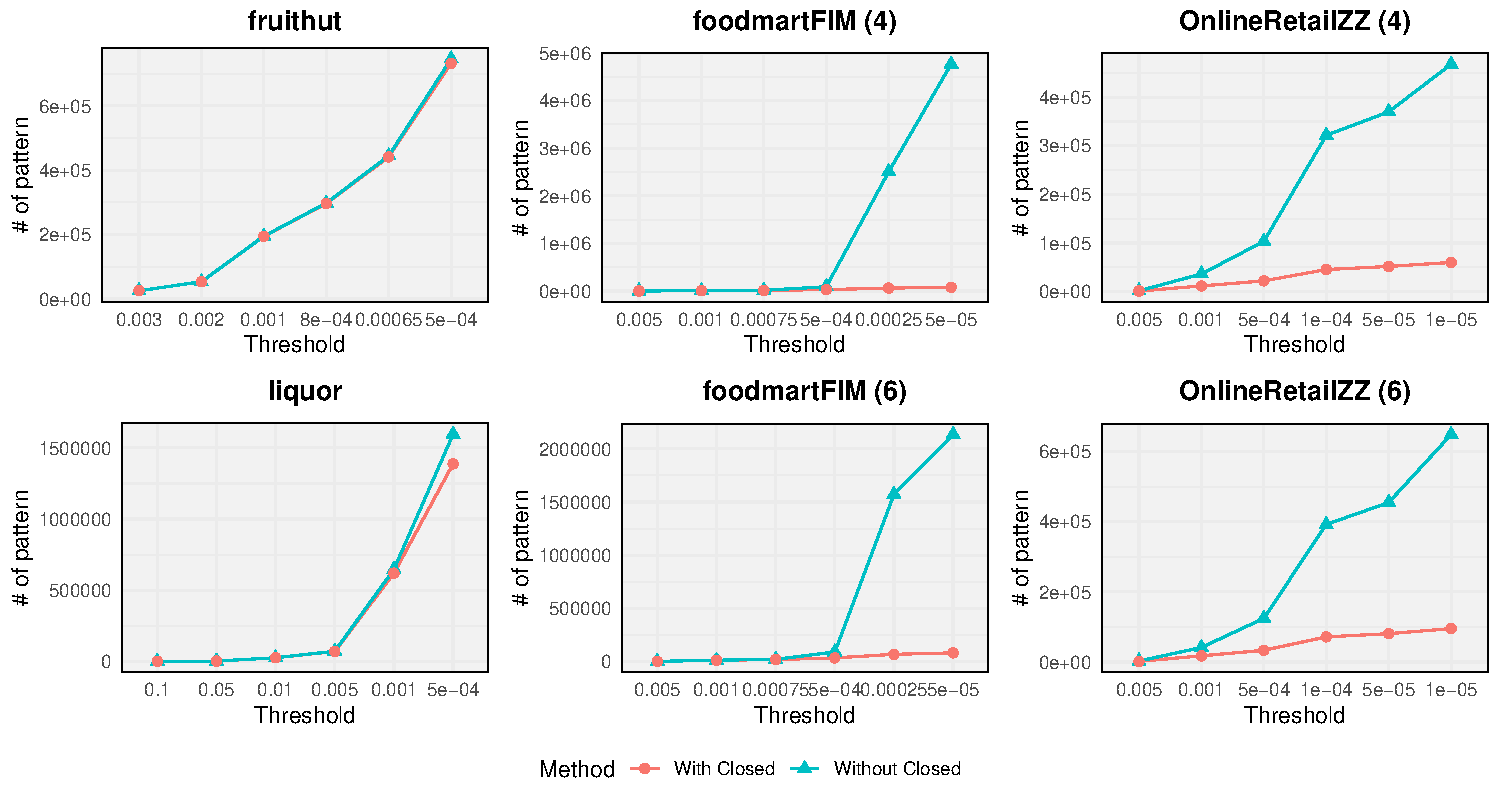
\includegraphics[width=0.8\textwidth]{closed_number_dense.pdf}
	% 標題務必簡潔明瞭，並且能夠清楚地描述圖表的內容和意義，讓讀者能夠快速理解圖表所傳達的信息。
	\caption{Example 1}
	\label{fig:chart1}
\end{figure}

\begin{figure}[ht]
	\centering
	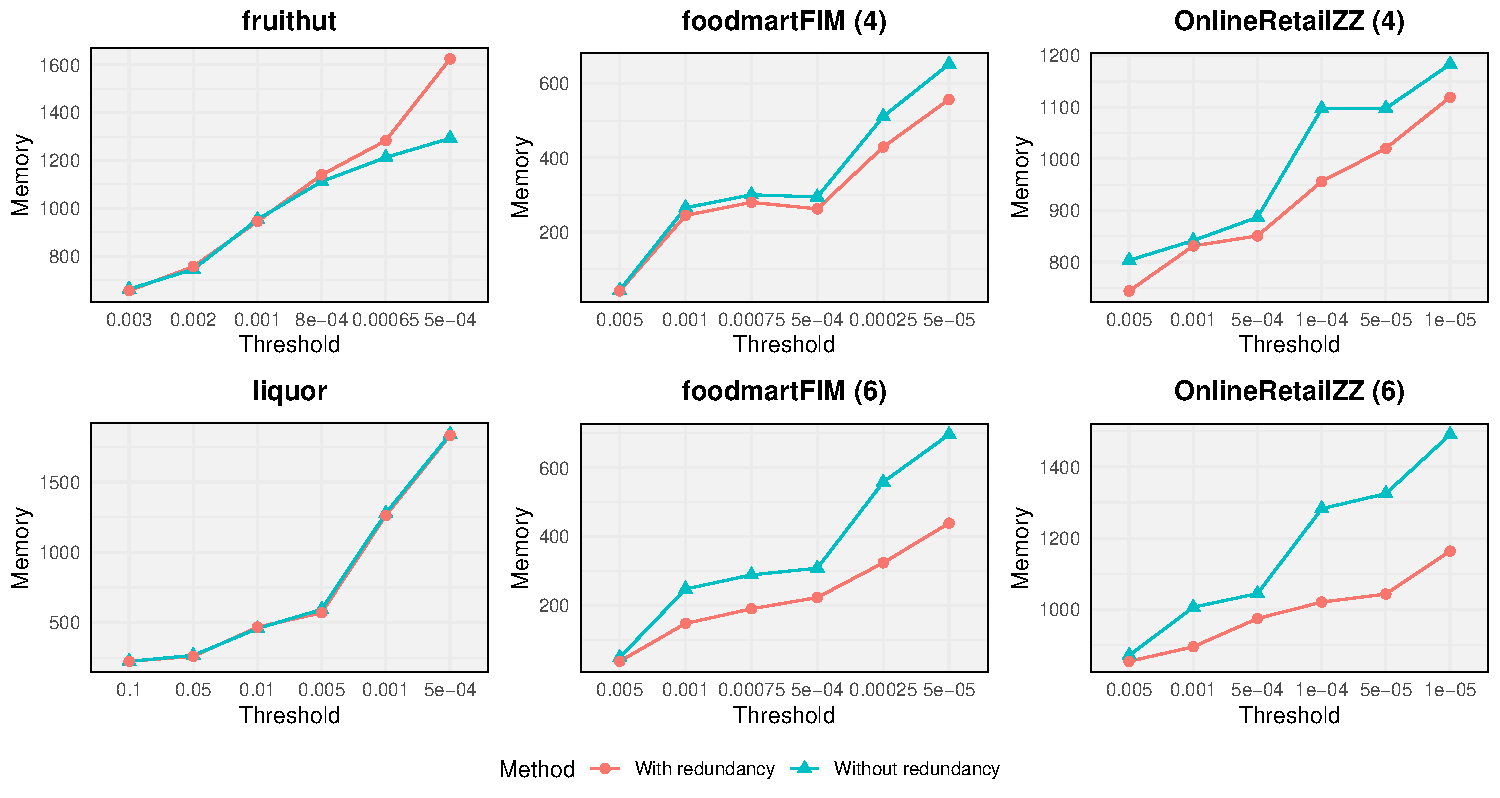
\includegraphics[width=0.8\textwidth]{redundancy_memory_dense.pdf}
	\caption{Example 2}
	\label{fig:chart2}
\end{figure}

% usepackage{algorithm} 和 usepackage{algpseudocode} 範例，提供了撰寫演算法的環境，讓我們能夠以清晰且結構化的方式展示我們的方法。
% 請務必使用 algpseudocode 來撰寫演算法，這樣可以確保演算法的格式統一且易於閱讀。
% 自定義關鍵字加粗 (Optional)
% \renewcommand{\algorithmicrequire}{\textbf{Input:}}
% \renewcommand{\algorithmicensure}{\textbf{Output:}}
\begin{algorithm}[ht]
	\caption{Parallel Data Mining Framework (WMT-Core)}
	\label{alg:wmt_parallel}
	\begin{algorithmic}[1] % [1] 表示每一行都標上行號
		\Require $D$: Large-scale dataset, $W$: Worker count
		\Ensure $R$: Refined insights

		\Function{WMTMining}{$D, W$}
		\State Initialize $Channels \gets \text{MakeChannels}(W)$ \Comment{Go-style concurrency}
		% \To 是自定義的關鍵字，已經在 preamble 區塊中定義了 \algnewcommand{\To}{\textbf{to }}，這樣在演算法中使用 \To 就會顯示為加粗的 "to "，提升了演算法的可讀性和專業性。
		% 請依照需要修改自定義的關鍵字，讓它們更符合你的演算法描述風格。
		\For{$i = 1$ \To $W$}
		\State \textbf{spawn} \Call{ProcessChunk}{$D_i, Channels[i]$} \Comment{Parallel execution}
		\EndFor

		\State $R \gets \emptyset$
		\While{not all channels empty}
		\State $data \gets \Call{Receive}{Channels}$
		\State $R \gets R \cup \Call{Aggregate}{data}$
		\EndWhile
		\State \Return $R$
		\EndFunction
	\end{algorithmic}
\end{algorithm}

% 結合 cleveref 引用
As detailed in \cref{alg:wmt_parallel}, our framework optimizes CPU utilization.


\section{Methodology}
We utilize the \texttt{tabularray} package to typeset professional-grade tables with a CSS-like syntax. As shown in Table \ref{tab:results}, the WMT algorithm achieves superior performance compared to the baseline.

\begin{table}[ht]
	\centering
	\caption{Experimental Results and Performance Comparison}
	\begin{tblr}{
			rows = {m}, columns = {c},
			row{1} = {font=\bfseries, gray9}, % 第一列加粗並給予背景色(Optional)
		}
		\hline[0.08em]
		Method   & Accuracy        & Latency       \\ \hline[0.05em]
		WMT-Algo & \textbf{98.5\%} & \unit{12}{ms} \\
		Baseline & 92.1\%          & \unit{45}{ms} \\ \hline[0.08em]
	\end{tblr}
	\label{tab:results}
\end{table}

\section{Future Work}
As a professor at the National Kaohsiung University of Science and Technology, I aim to integrate these automated typesetting tools into our laboratory's standard operating procedures. This approach ensures that our research outputs meet the highest publication standards.

% 引用 references.bib 中的文獻
% 注意，製作 bib 檔時請確保格式統一且完整，特別是作者姓名、文章標題、期刊名稱、卷號、頁碼和出版年份等關鍵信息，這樣才能確保在生成參考文獻列表時能夠正確顯示。
% 我的習慣是，論文 title 的第一個字母 (或是冒號:後面的第一個字母) 大寫，其他字母小寫，除非是專有名詞或者縮寫，這樣能夠保持參考文獻列表的整潔和一致性。
% 期刊或是 Proceedings 的名稱則是每個單字的第一個字母都大寫 (連接詞例外)，這樣能夠突出期刊或會議的名稱，讓讀者更容易識別。
% 自動生成參考文獻列表
\printbibliography

\end{document}
